\iffalse
\documentclass{article}
% Language setting
% Replace `english' with e.g. `spanish' to change the document language
\usepackage[english]{babel}
% Set page size and margins
% Replace `letterpaper' with `a4paper' for UK/EU standard size
\usepackage[letterpaper,top=2cm,bottom=2cm,left=3cm,right=3cm,marginparwidth=1.75cm]{geometry}
% Useful packages
\usepackage{multicol}
\usepackage{amsmath}
\usepackage{amssymb}
\usepackage{graphicx}
\usepackage[framemethod=tikz]{mdframed}
\usepackage{array}
\usepackage{blindtext}
%\usepackage[paperwidth=10cm]{geometry}
\usepackage{tkz-euclide}
%\usepackage{tikz}
\usetikzlibrary{
  circuits.logic,
  circuits.logic.US,
  positioning
}

\usepackage[colorlinks=true, allcolors=blue]{hyperref}
\newcommand{\myvec}[1]{\ensuremath{\begin{pmatrix}#1\end{pmatrix}}}
\providecommand{\norm}[1]{\left\lVert#1\right\rVert}
\let\vec\mathbf
\title{Optimization Assignment-1}
\author{Thoutu Rahul Raj}
\begin{document}
\maketitle
\newtheorem{theorem}{Theorem}[section]
\begin{multicols}{2}

\paragraph{\begin{flushleft}\textbf{Problem: }
	\fi
Minimise
	\begin{align}
Z = -3x+4y 
\end{align}
such that 
\begin{align}
	x+2y &< 8,\\
	3x+2y &< 12,\\
	x > 0, y &>  0
\end{align}
\\
\solution
	\begin{figure}[!ht]
		\centering
		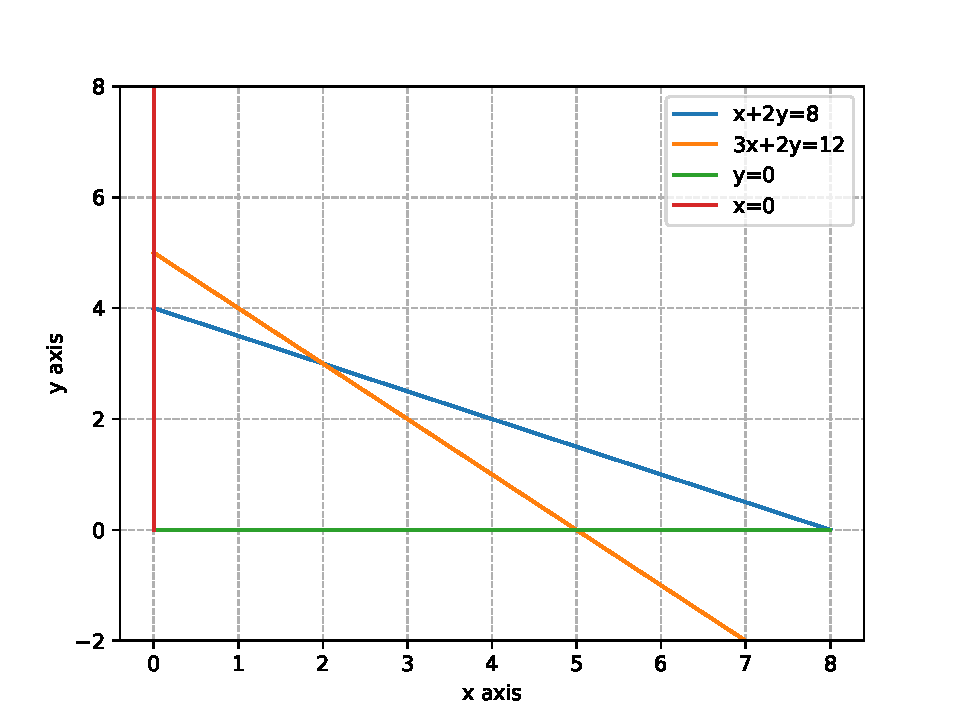
\includegraphics[width=\columnwidth]{12/12/1/2/figs/fig.pdf}
		\caption{}
		\label{fig:12/12/1/2}
  	\end{figure}
	\iffalse
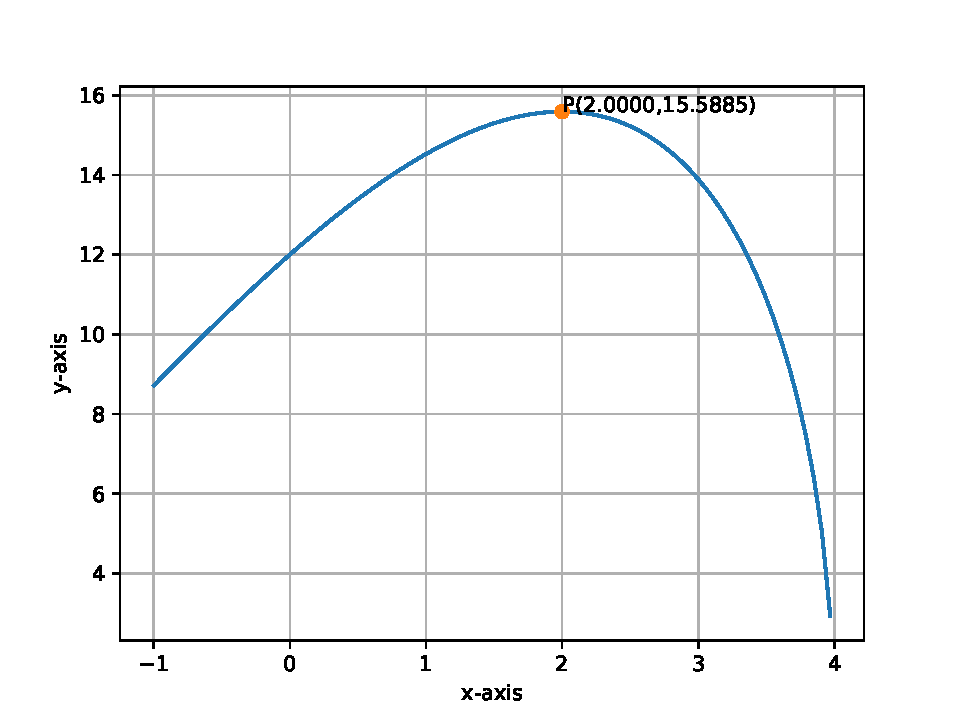
\includegraphics[scale=0.5]{fig.pdf} 
\end{flushleft}}
\section*{Solution}
\begin{flushleft}
	\fi
	The given
problem can be formulated as
\iffalse
\begin{align}
\min_{\vec{x}} Z=(-3x+4y)
\end{align}
\begin{align}
x+2y \preceq8
\end{align}
\begin{align}
3x+2y \preceq 12
\end{align}
\begin{align}
x\succeq0,y\succeq0
\end{align}
eq 2 and 3 to 4 can be expressed in vector form as
\fi
\begin{align}
	\min_{\vec{x}}Z=\myvec{-3 & 4}\vec{x}\\
\myvec{1 & 2\\
       3 & 2\\
       1 &0\\
       0 & 1}\vec{x}\succeq \myvec{8 \\12\\0\\0}
\end{align}
Solving above equations using cvxpy, we get
\begin{align}
	\min_{\vec{x}} Z&=-12
	\\
	\vec{x}&=\myvec{4\\0}
\end{align}
